\chapter{Results}

	In this chapter the results of GPU design choices and algorithmic
	optimizations and their effects are reviewed.

	\section{Software Shader Performance}

		The shader performed as expected, a conventional graphics card is
		capable of rendering scenes with low scene complexity in real-time
		using sphere tracing.

		Scenes can easily be made to look a lot more complex than they
		are, for example, by using mod fields, when the modulo
		operation is used on an object it creates a field with multiple copies
		of the original object next to each other, or fractals. The hardware
		(Geforce GTX 1060M) that the shader was tested on was able to render 20
		reflective spheres in real time in fullHD using our performance
		enhancing algorithm.
 
	\section{GPU}
	
		The GPU has been tested by simulating it and running a program on the simulation 
		that renders a sphere using Sphere Tracing. It spawns threads
		progressively to fill the screen data buffer with pixels. The execution
		of our test programs ran exactly as intended, with any number of
		simulated cores. The design has also been put through a synthesizing
		tool for FPGAs, which creates a net list of the components and
		connections that constitute the GPU. This also works as intended
		without any unexpected problems, but the actual operation of the GPU on
		an FPGA has not yet been verified.
	
	\section{Square roots}
		
		The accuracy of the different square root approximation and calculation
		methods are shown in figures \ref{sres1}, \ref{sres2}, \ref{sres3},
		\ref{sres4}, \ref{sres5}, and \ref{sres6}. The shifting nth root
		algorithm is used as a reference in all figures because it is always
		bit-accurate for integer square roots.

		\begin{figure}[H]
			\centering
			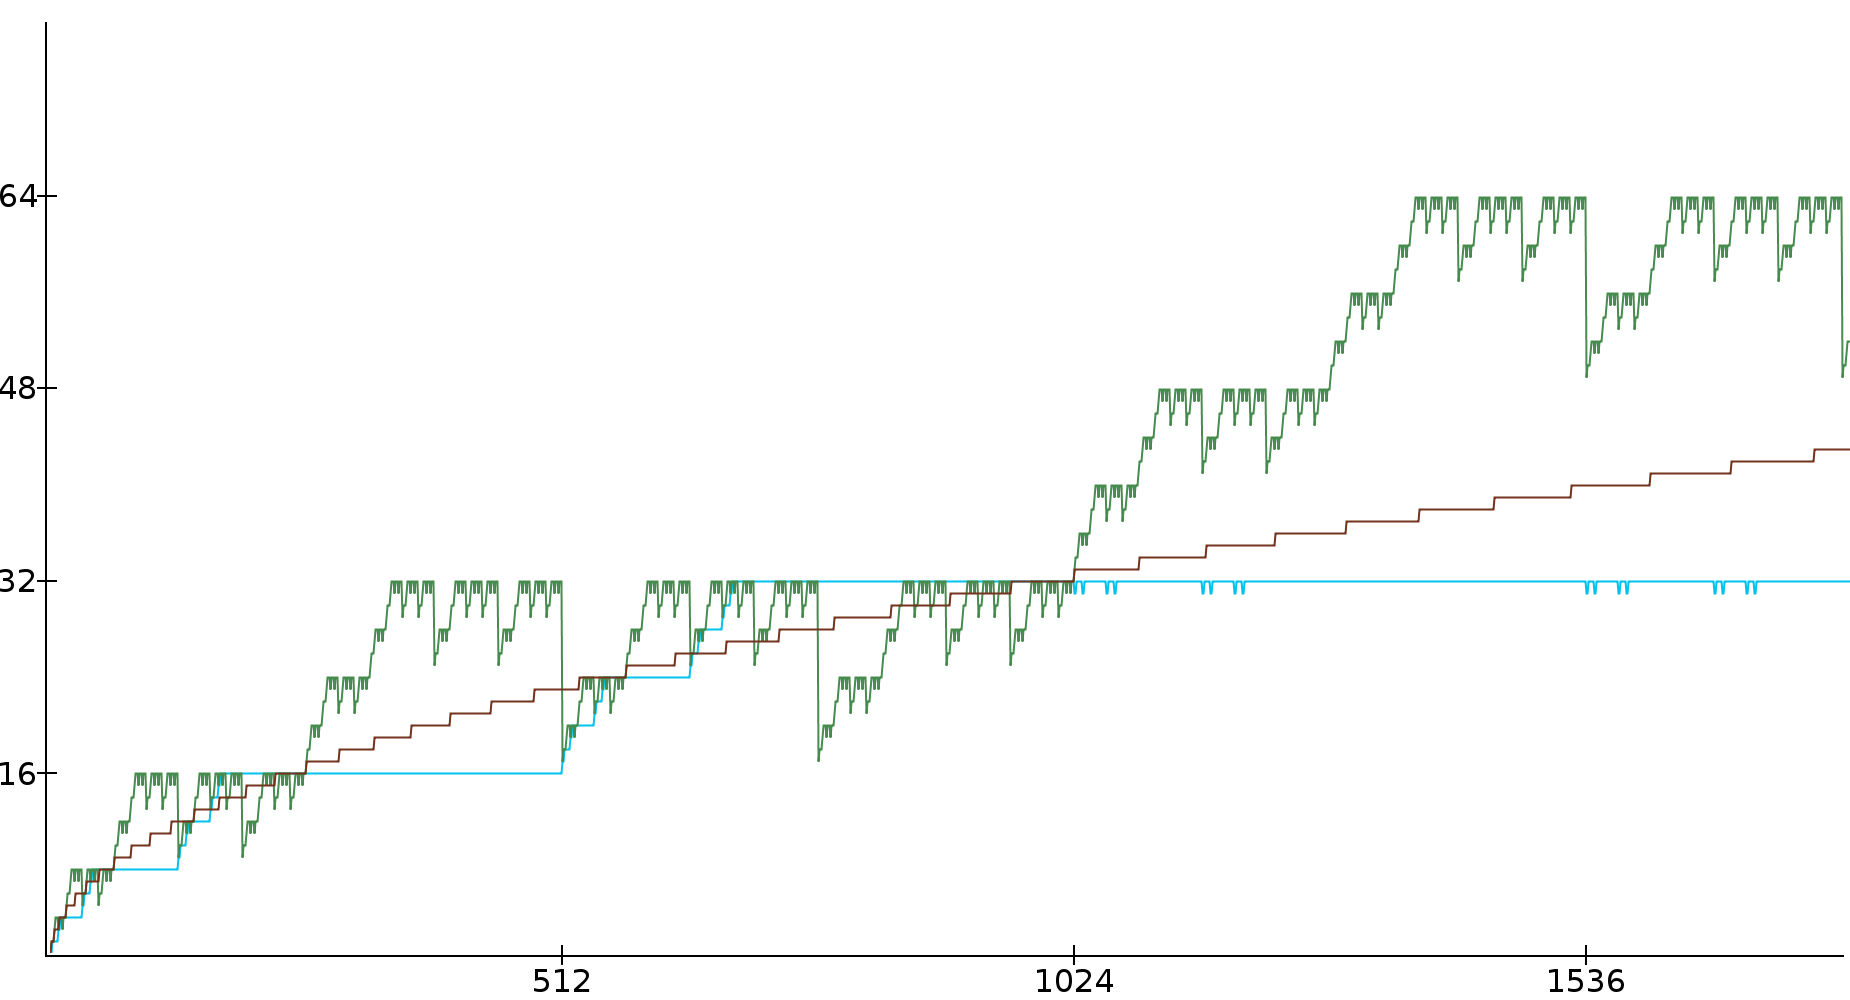
\includegraphics[width=0.75\linewidth]{figure/value12x.png} 
			\caption{Value from the simple square root approximator (green),
				the improved version (blue), and the shifting nth root 
				algorithm (red). In these graphs, they all operate on integers. 
				The shifting nth root is exact for integer square roots.}
			\label{sres1}
		\end{figure}

		\begin{figure}[H]
			\centering
			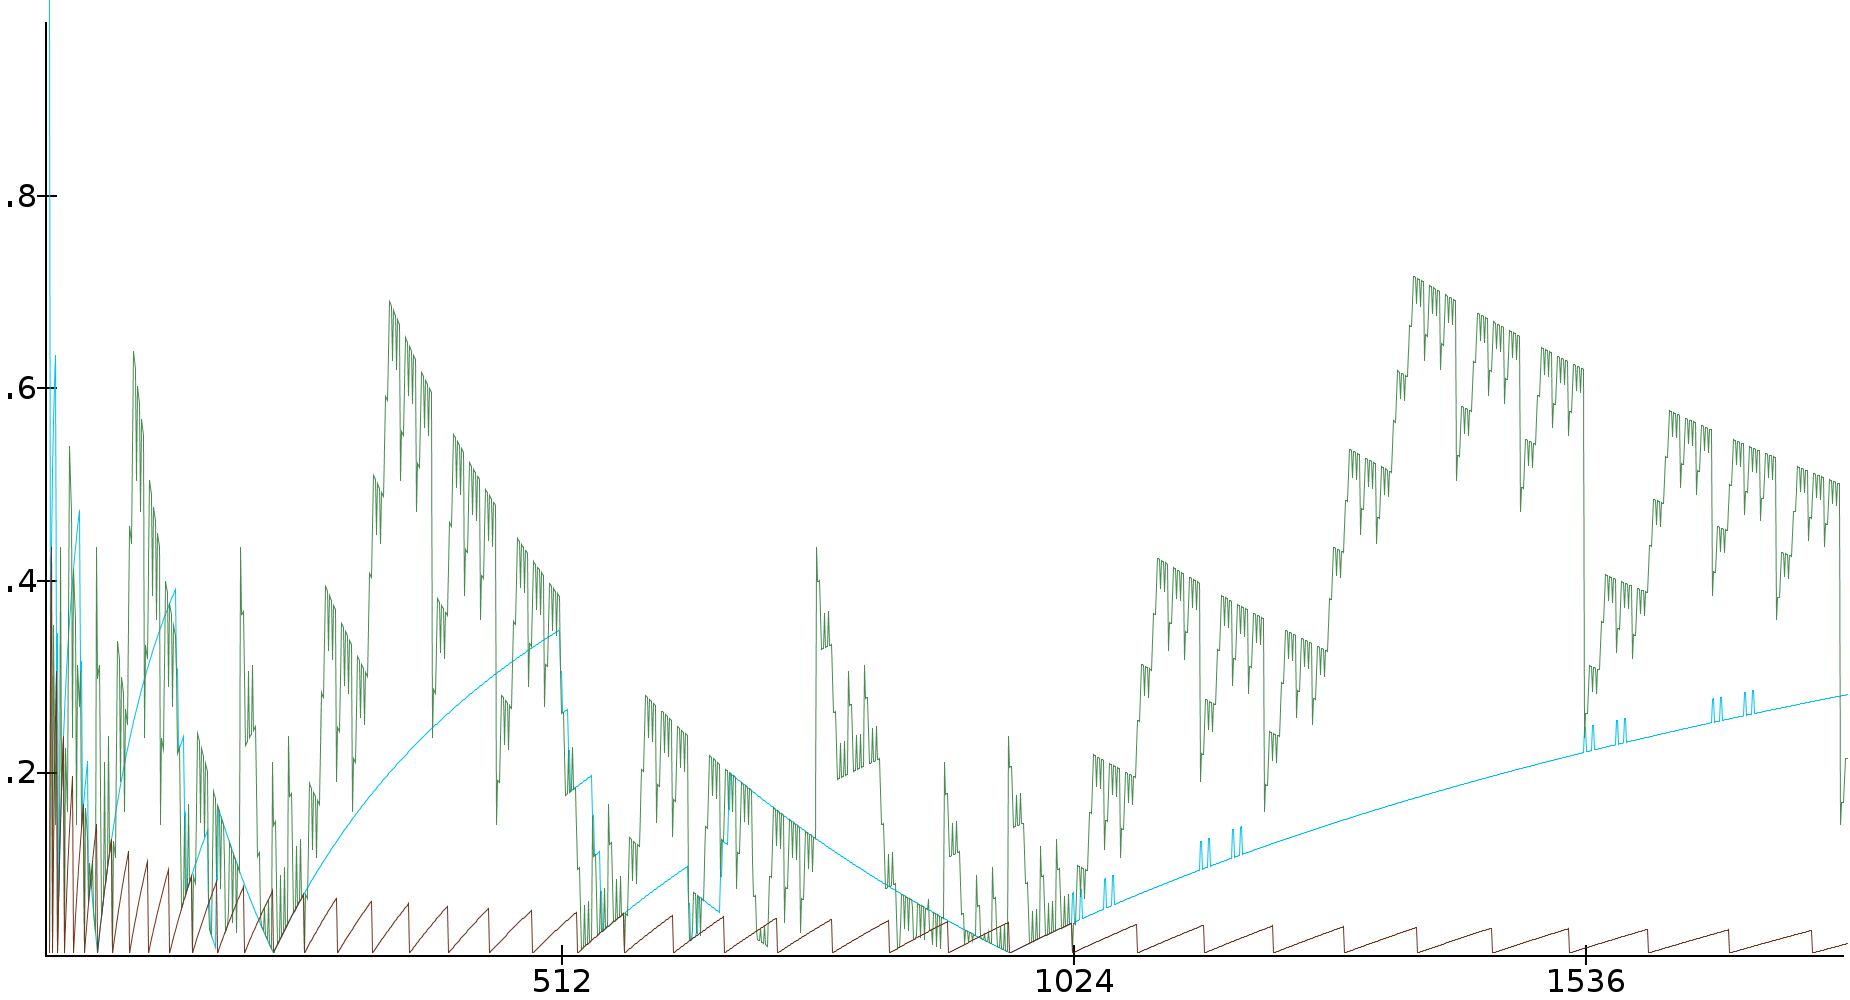
\includegraphics[width=0.75\linewidth]{figure/rel_error_480x.png} 
			\caption{Relative error for the simple square root approximator
				(green), the improved version (blue), and the shifting nth root
				algorithm (red).}
			\label{sres2}
		\end{figure}

		\begin{figure}[H]
			\centering
			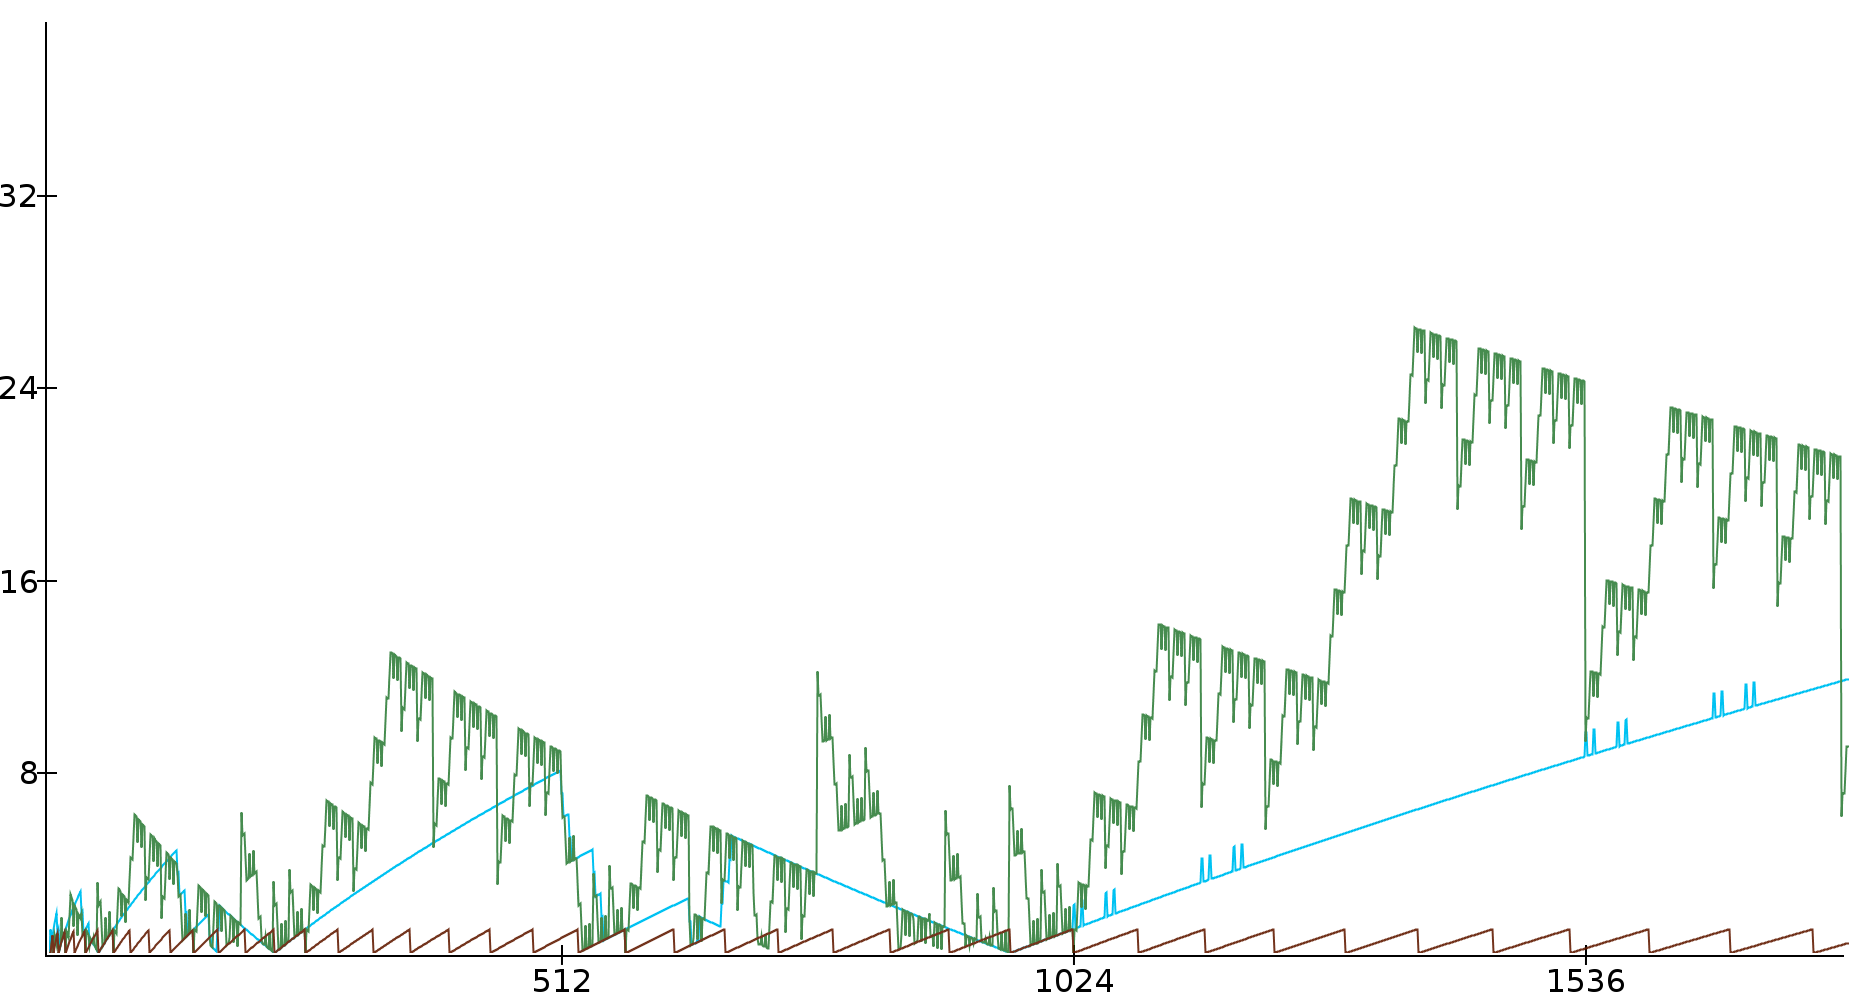
\includegraphics[width=0.75\linewidth]{figure/abs_error_24x.png} 
			\caption{Absolute error for the simple square root approximator
				(green), the improved version (blue), and the shifting nth root
				algorithm (red).}
			\label{sres3}
		\end{figure}

		\begin{figure}[H]
			\centering
			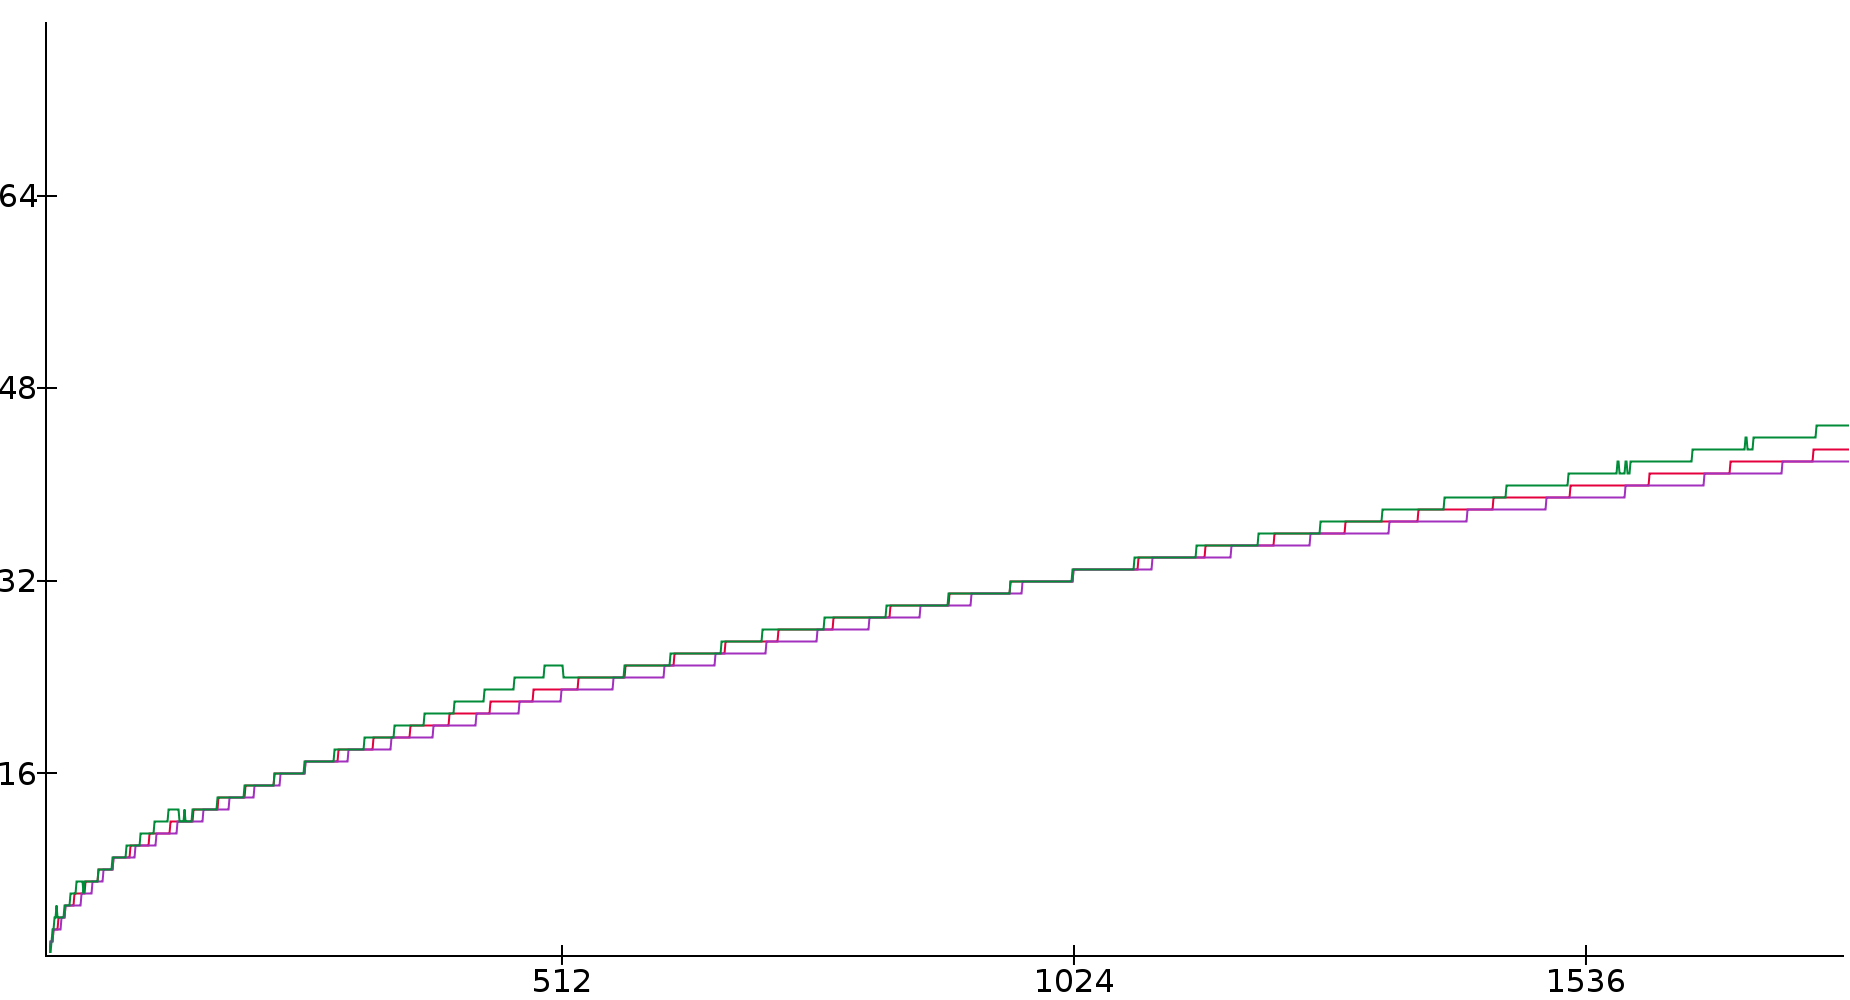
\includegraphics[width=0.75\linewidth]{figure/value_lin12x.png} 
			\caption{Value from lerp-approximator (purple), simple square root
				approximator with one step of the babylonian method (green),
				and the shifting nth root algorithm (red). In these graphs, 
				they all operate on integers. The shifting nth root is exact 
				for integer square roots.}
			\label{sres4}
		\end{figure}

		\begin{figure}[H]
			\centering
			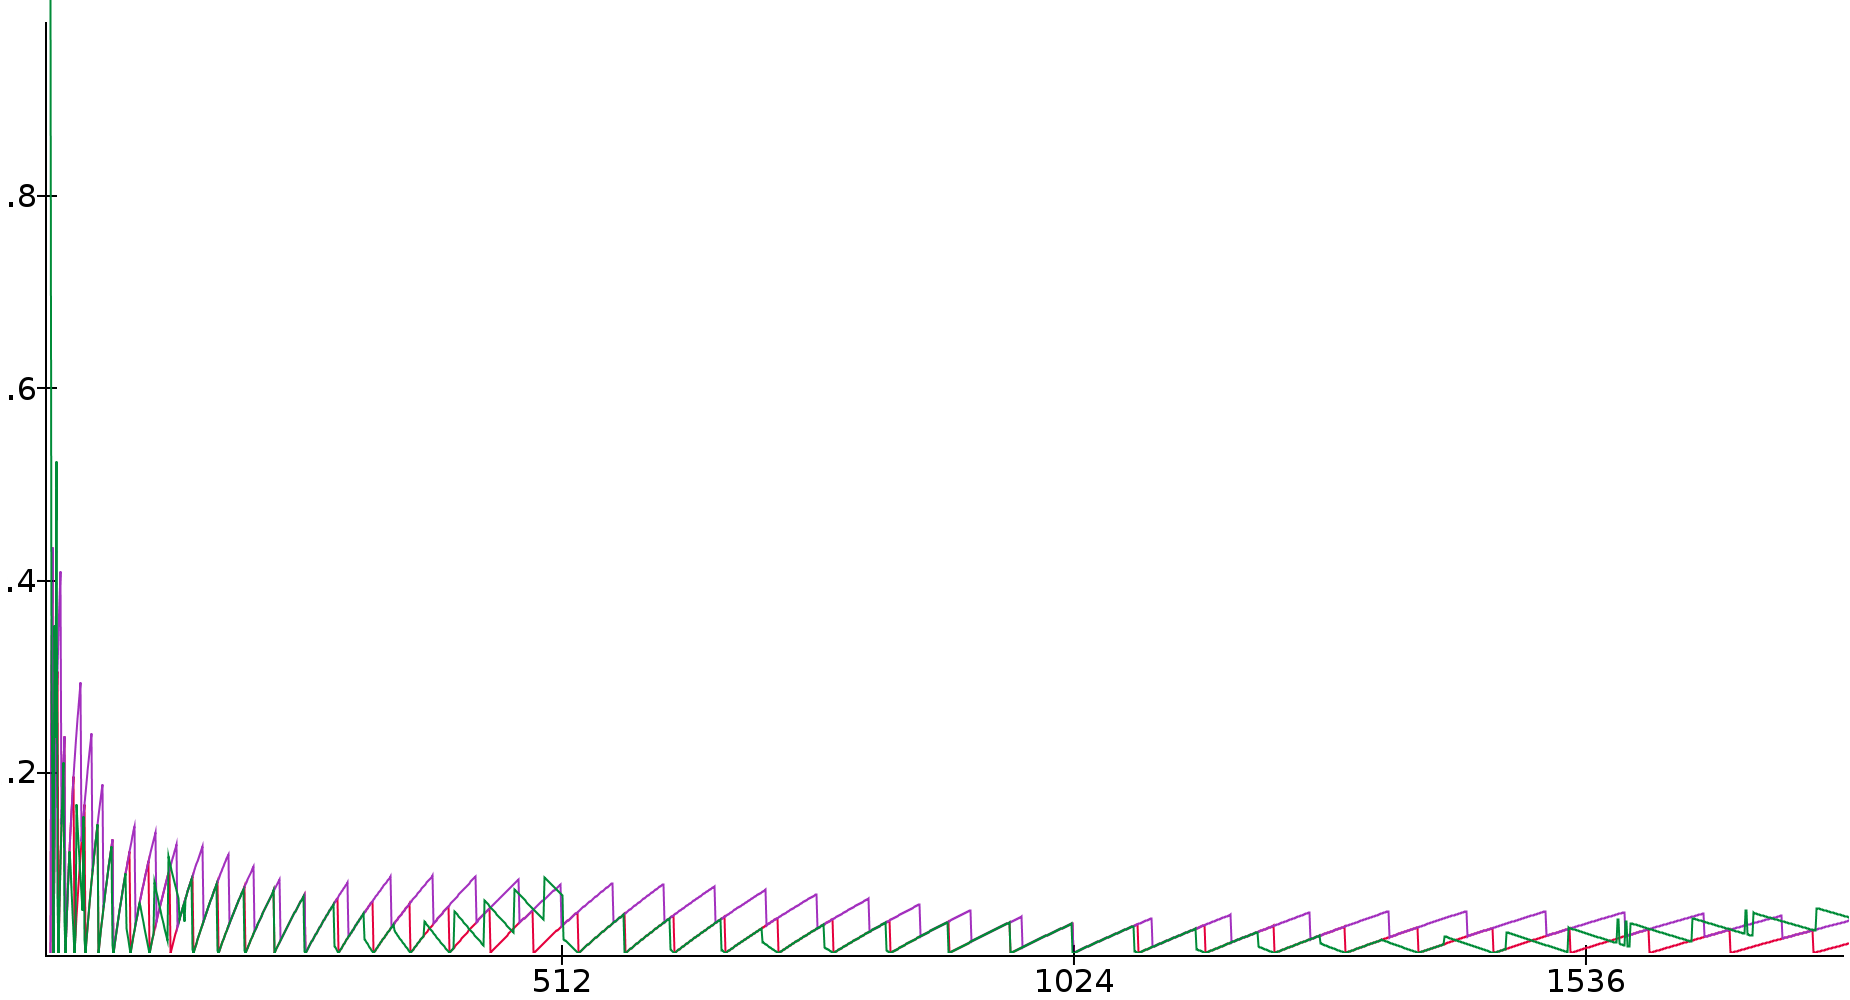
\includegraphics[width=0.75\linewidth]{figure/rel_lin960x.png} 
			\caption{Relative error for the lerp-approximator (purple), simple 
				square root approximator with one step of the babylonian method 
				(green), and the shifting nth root algorithm (red).}
			\label{sres5}
		\end{figure}

		\begin{figure}[H]
			\centering
			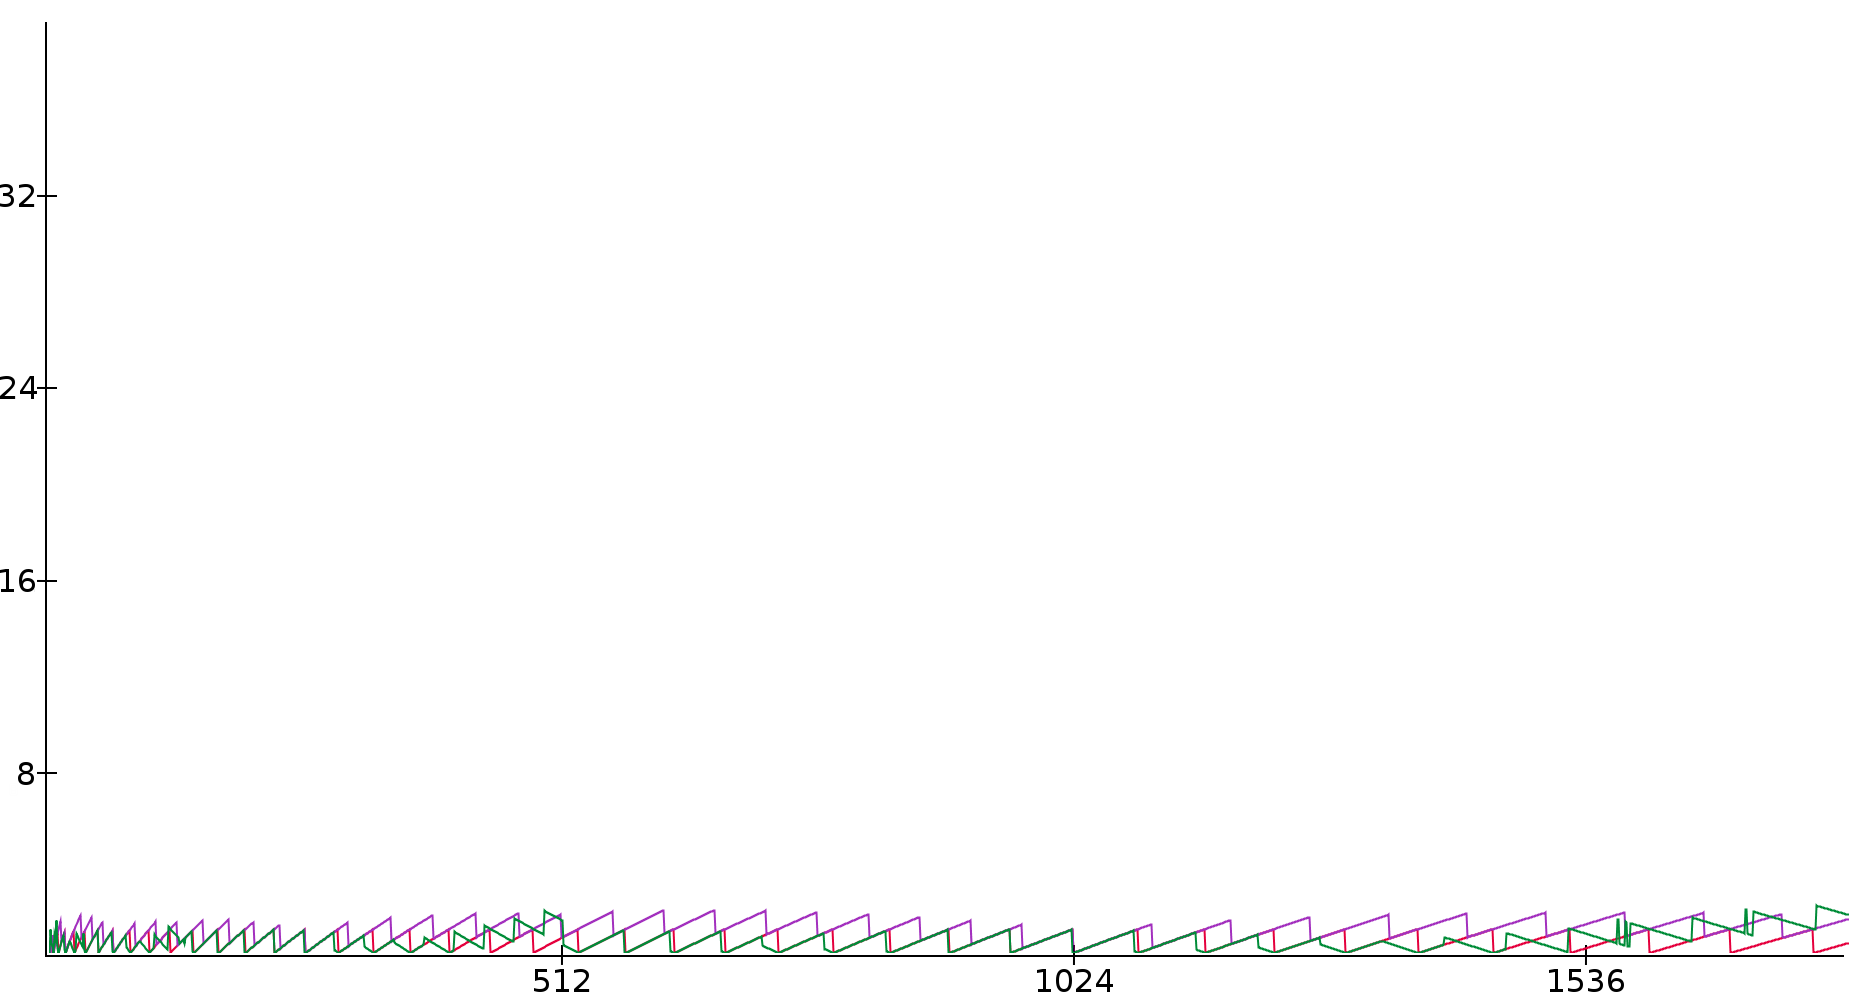
\includegraphics[width=0.75\linewidth]{figure/abs_lin24x.png} 
			\caption{Absolute error for the lerp-approximator (purple), simple 
				square root approximator with one step of the babylonian method 
				(green), and the shifting nth root algorithm (red).}
			\label{sres6}
		\end{figure}

	\section{Optimizations}
		
		During this project, a number of optimizations were discussed and
		developed. Implemented optimizations are explained below and the
		theoretical ones are presented in chapter \ref{discussion} and
		\ref{optimization}. Some of these are based on earlier work, while
		others are believed to be quite unique optimizations which have not been
		discussed for sphere tracing previously. All implemented optimizations
		that affects the algorithm were implemented in the software shader, not
		on our own GPU.

		For all tests performed, FPS (Frames Per Second) is used to measure
		performance. FPS is simply how many times the GPU is able to render 
		the scene per second. The time it takes to render the scene once is 
		equal to one divided by the FPS.

		\subsection{Orthogonal culling}
		
		Tests to see the performance of the Orthogonal Culling optimization
		were performed by putting an increasing number of solid-colored spheres
		in a plane in front of the camera. Because of this, the spheres are not
		obstructed by other spheres, making this the best possible scenario for
		the optimization.

		Below are test results from Orthogonal culling.

			\begin{table}
			\centering
			\begin{tabular}{lll}
				\hline
				Objects & Optimized & Unoptimized \\ 
				\hline
				1       & 600       & 350         \\ 
				5       & 430       & 180         \\			
				10      & 290       & 98          \\
				15      & 85        & 13          \\
				20      & 58        & 9           \\
				25      & 40        & 6           \\
				30      & 29        & 4           \\
				35      & 7         & 3           \\
				40      & 6         & 2           \\
				45      & 4         & 1.5         \\
				\hline
			\end{tabular}
			\caption{Frames generated per second using the GLSL shader with and
				without the orthogonal culling optimization.}
			\end{table}

			\begin{figure}[H]
				\centering
				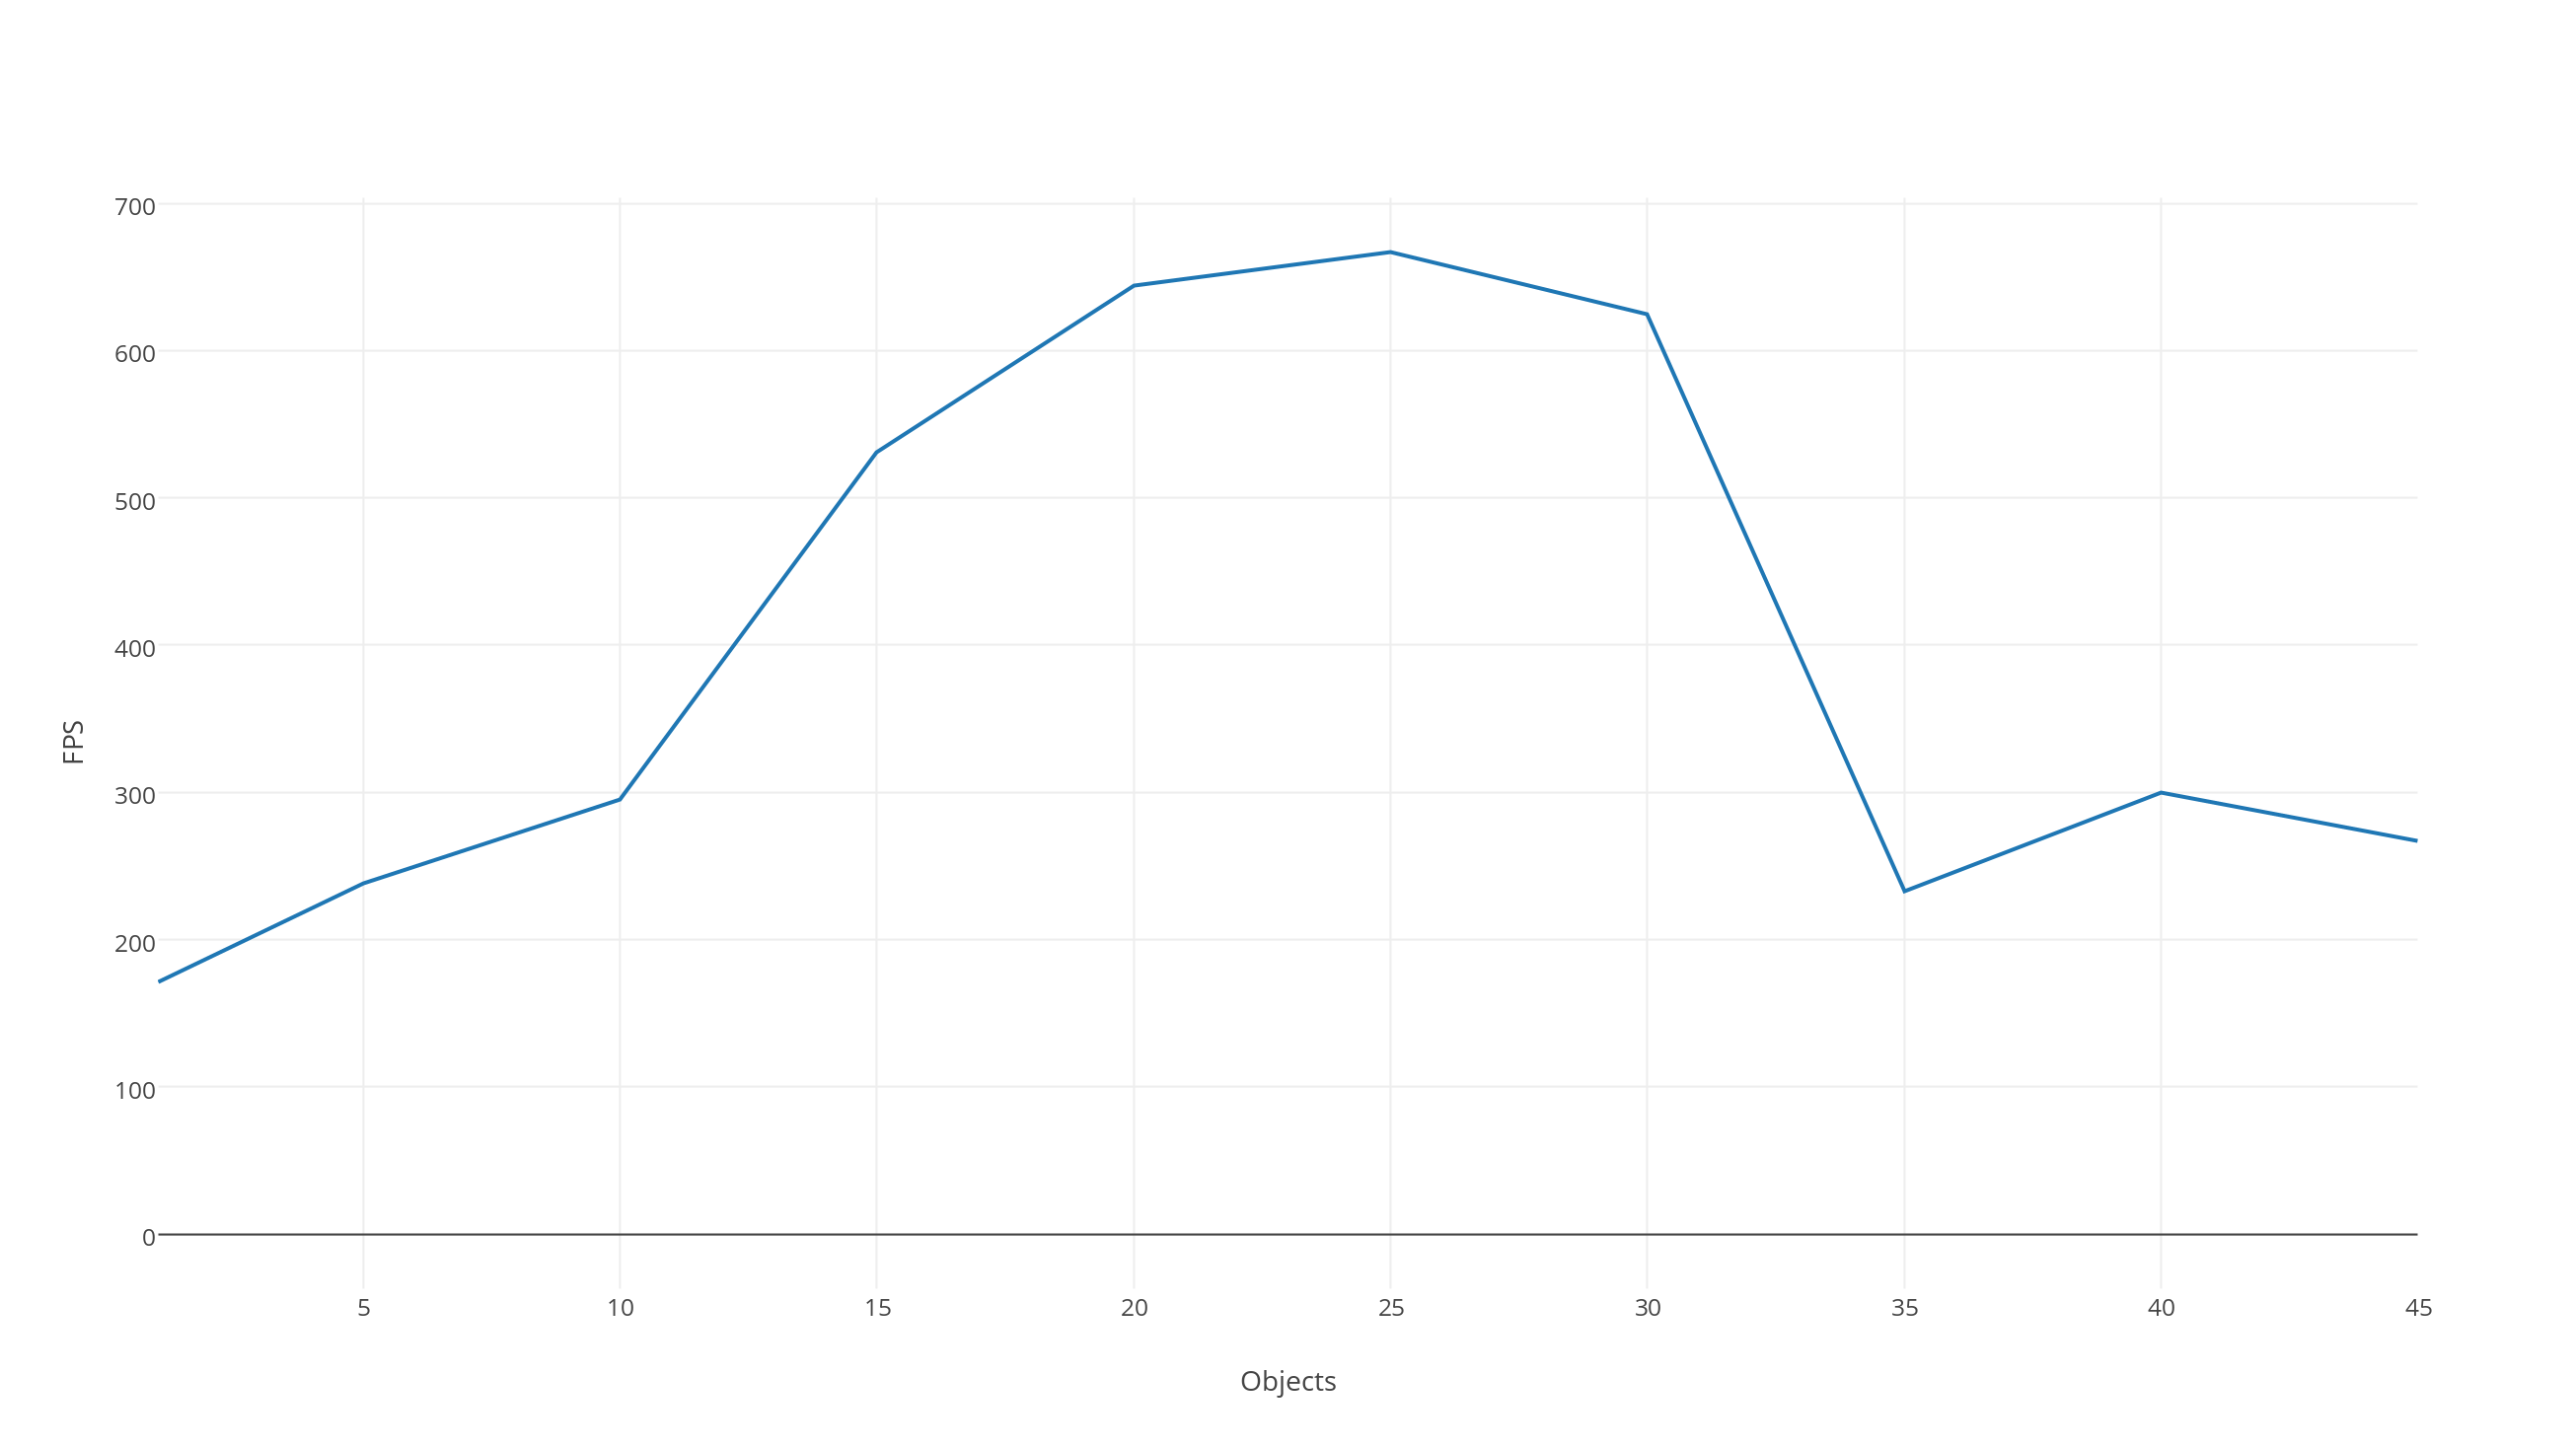
\includegraphics[width=1.0\linewidth]{figure/TestResults/PercentageImprovement.png} 
				\caption{Results from Orthogonal Culling tests. The reason for this graph's irregular behavior is probably some 
			instruction memory cache running out or something of that 
			fashion, although we can't know for sure. }
				\label{orthcull}
			\end{figure}



		\subsection{Bounding spheres}

			Bounding spheres were implemented and tested. There was a clear
			gain in performance in some cases, but the results are situational. 
			The performance gain depends on number of objects bound, the spacing
			between them, how well the sphere fits the objects, etc. 

			To test the performance of this method a scene with an successively 
			increasing amount spheres was rendered and the FPS measured. For 
			reference an identical scene was rendered but without the 
			optimization running.

			\begin{figure}[H]
				\centering
				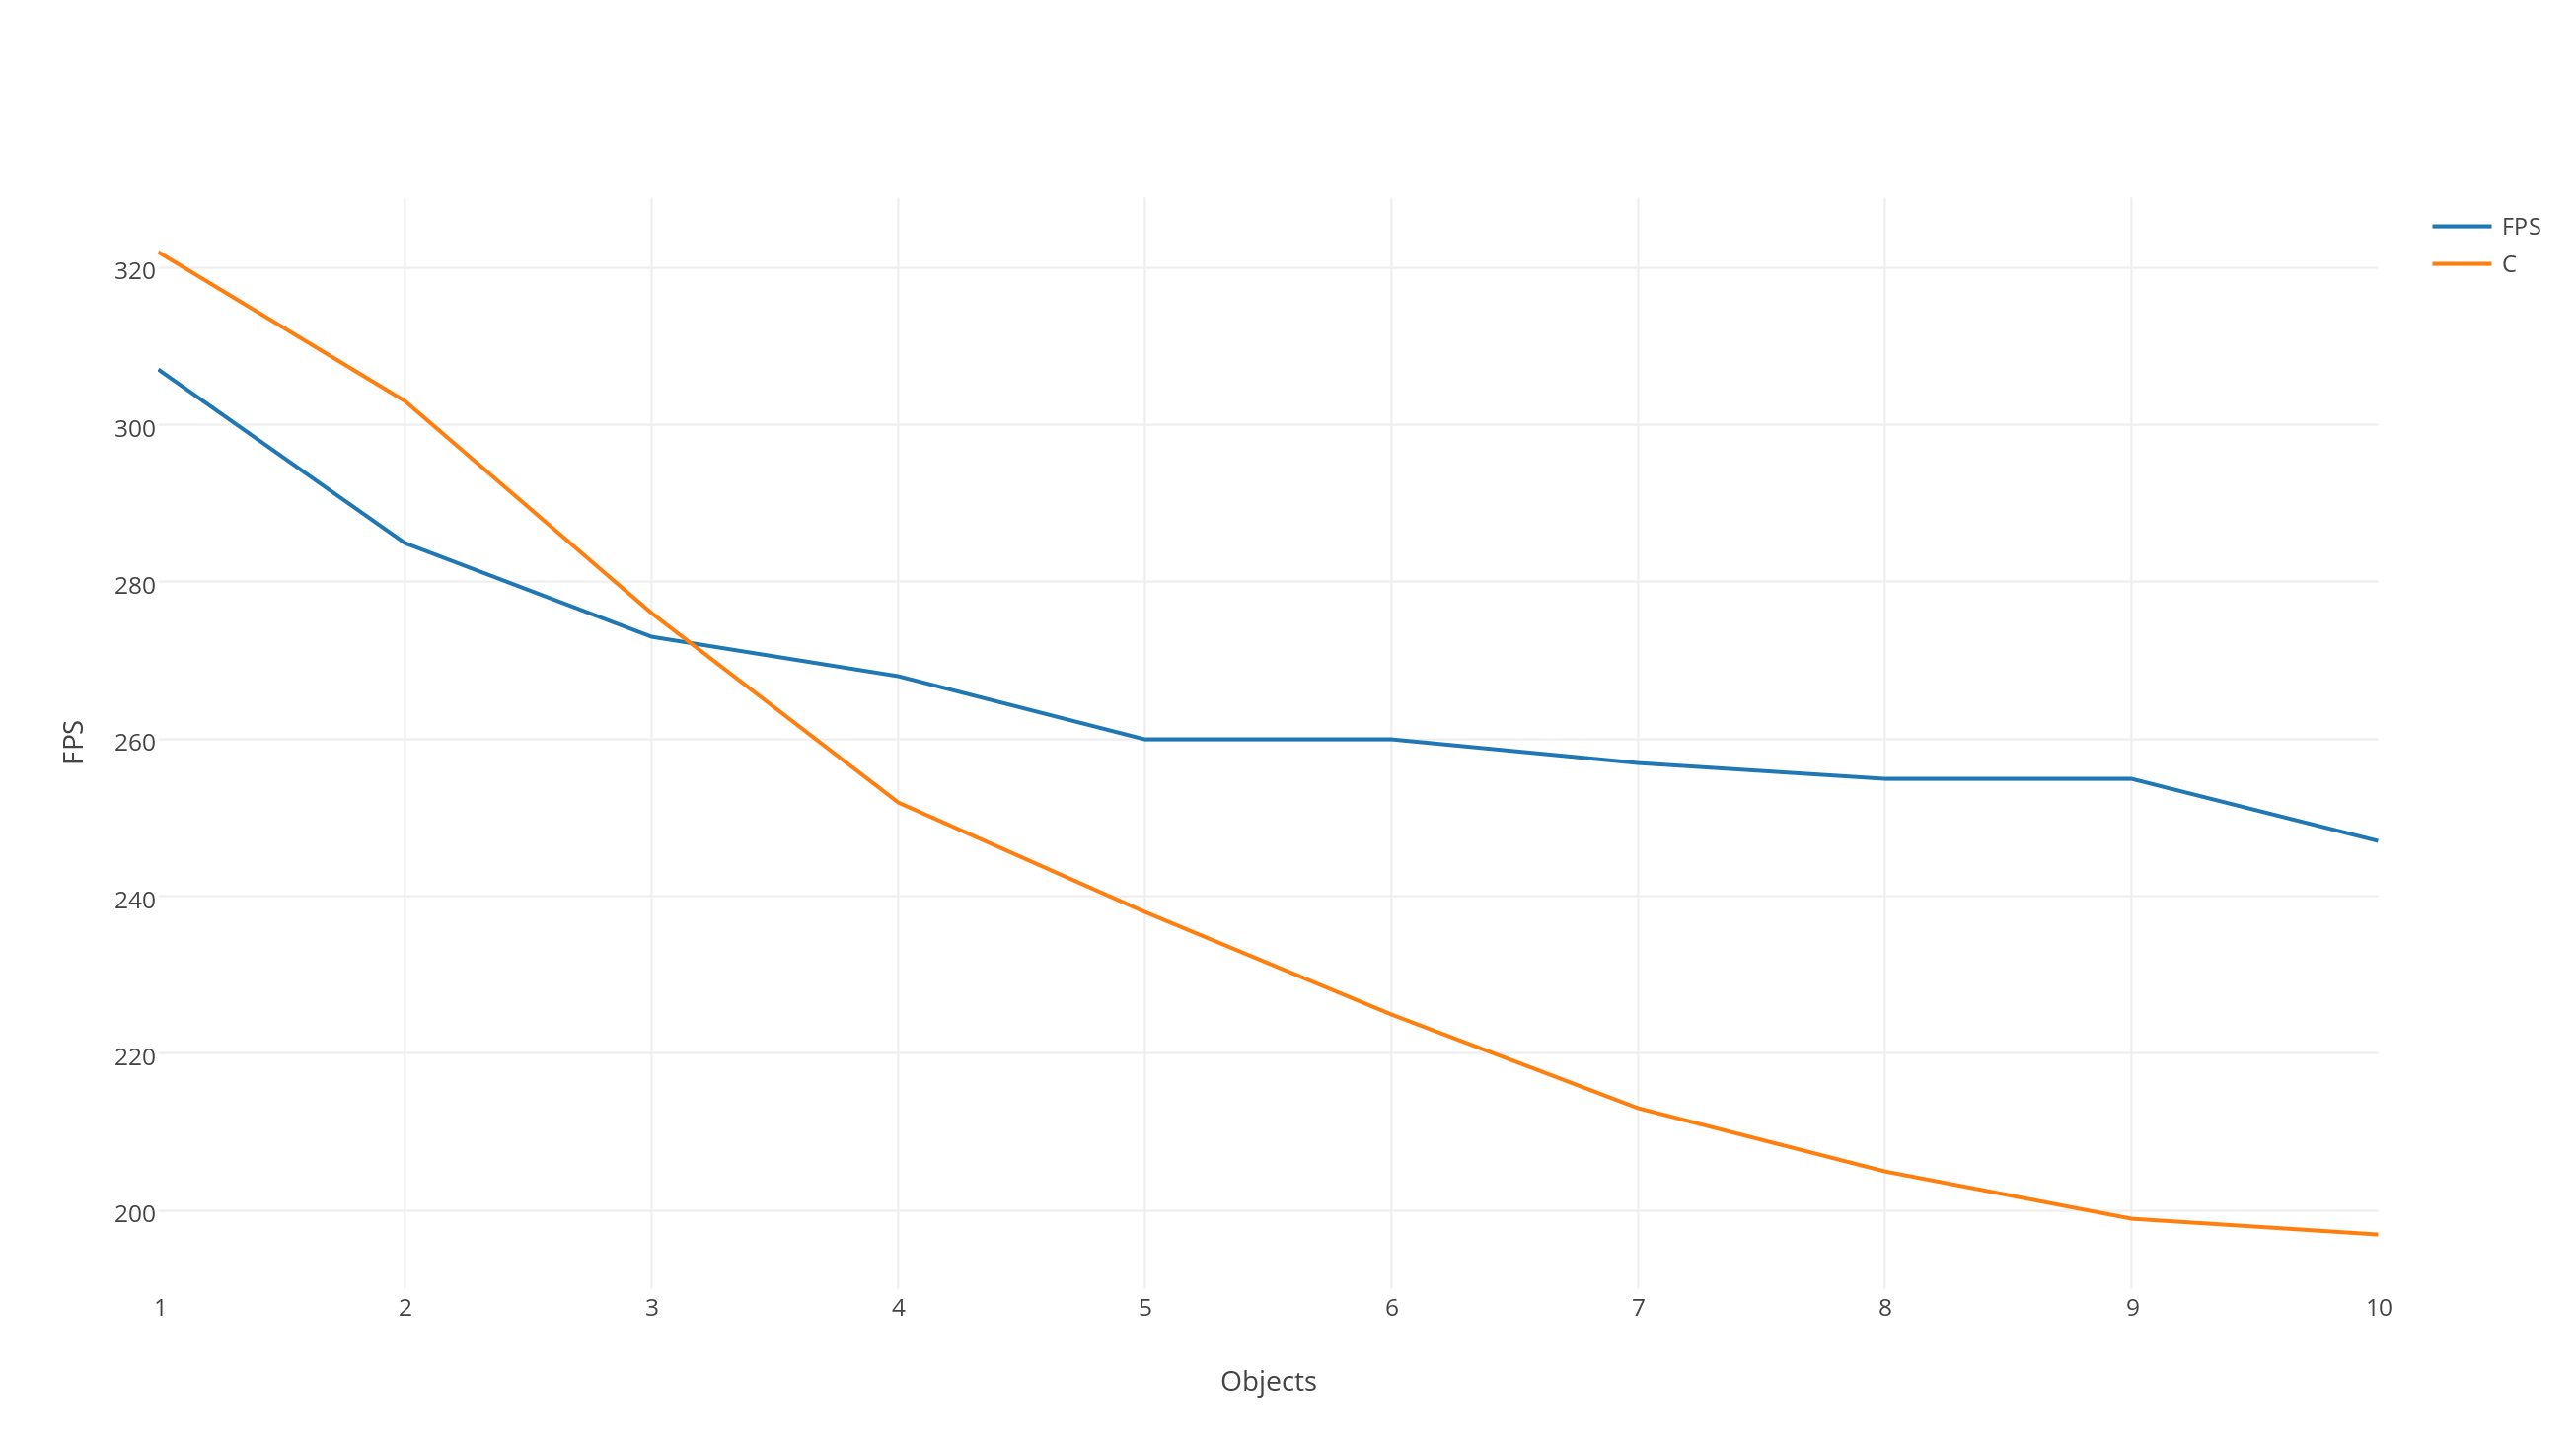
\includegraphics[width=1.0\linewidth]{figure/TestResults/BSObjects.png} 
				\caption{Results from Bounding Sphere test. Blue is optimized, red is without optimization}
				\label{boundsphere}
			\end{figure}

			This chart shows that in this scene a performance gain is observed 
			when more than three objects are placed in a Bounding Sphere. If
			fewer than 4 objects are enclosed, a performance decrease is 
			observed.
